\section{Zarządzanie wątkami – tworzenie, kończenie, atrybuty wątków}

\subsection{Wprowadzenie}

Podczas rozwoju oprogramowania, np. czasu rzeczywistego, wbudowanego, graficznego, często zachodzi potrzeba przetwarzania współbieżnego, bądź równoległego, w przypadku implementacji na komputerach równoległych z~pamięcią wspólną. Współbieżność (równoległość) tę można osiągnąć poprzez używanie wątków POSIX (biblioteka \lstinline[style=MyBashStyle]{pthread}), zaimplementowanych w~systemie QNX i~opartych na standardzie \lstinline[style=MyBashStyle]{IEEE POSIX 1003.1c}.

Dotyczczas zajmowaliśmy się procesami mającymi po jednym wątku. Pojęcie procesu można rozszerzyć do istnienia wielu wątków sterowania i~rozpatrywać proces jako zbiór wątków i zasobów. Wątek w~tym przypadku będzie traktowany jako elementarna, niezależna jednostka, podlegająca szeregowaniu (scheduling). Część zasobów procesu jest wspólna dla jego wszystkich wątków. Należą do nich:

\begin{myitemize}
\item Wspólna przestrzeń adresowa, w~szczególności zmienne statyczne i sterta.
\item Pliki i~urządzenia wejścia-wyjścia.
\item Kanały, kolejki i połączenia.
\end{myitemize}

Wątki mają również swoje prywatne atrybuty i~zasoby. Spośród ważniejszych można wymienić:

\begin{myitemize}
\item Identyfikator wątku TID (thread identifier).
\item Priorytet.
\item Stos.
\item Zestaw rejestrów.
\item Atrybuty służące szeregowaniu wątków.
\item Maska sygnałów.
\item Lokalne zmienne wątku TLS (thread local storage).
\item Procedura zakończenia wątku.
\end{myitemize}

Zalety stosowania wielowątkowego modelu programowania (multithreaded programming model):

\begin{myitemize}
\item Mniejszy koszt tworzenia, kończenia, w~porównaniu z~procesami.
\item Zwykle szybszy czas przełączenia wątków niż procesów.
\item Wszystkie wątki dzielą tę samą przestrzeń adresową. W~wielu przypadkach, komunikacja między wątkami jest łatwiejsza i~wydajniejsza, niż komunikacja międzyprocesorowa.
\item Korzyści wydajnościowe, w~przypadku przetwarzania równoległego na maszynach z pamięcią wspólną SMP (symmetric multiprocessing) - cecha szczególnie istotna, ze względu na fakt istnienia relatywnie tanich procesorów wielordzeniowych (multicore processors).
\end{myitemize}

Biblioteka pthread zawiera wiele funkcji, które umożliwiają zarządzanie wątkami. Ich prototypy zostały zdefiniowane w pliku nagłówkowym \lstinline[style=MyBashStyle]{pthread.h}.  Procedury można podzielić zgrubnie na trzy grupy:

\begin{myitemize}
\item Zarządzanie wątkami – tworzenie, anulowanie, odłączanie, dołączanie wątków, operowanie na atrybutach wątków.
\item Mechanizmy synchronizacji wątków (np. muteksy, zmienne warunkowe, bariery).
\item Mechanizmy komunikacji wątków.
\end{myitemize}

Biblioteka \lstinline[style=MyBashStyle]{pthread} zawiera ponad 60 procedur, zdefiniowanych dla języka~C. W~trakcie niniejszego laboratorium skupimy się na zbiorze funkcji, które są na ogół najczęściej używane i~będą użyteczne dla początkującego programisty wątków POSIX.

\subsection{Zarządzanie wątkami}
\subsubsection{Tworzenie wątków}

Funkcja \lstinline[style=MyCStyle]{main()} posiada jeden wątek (domyślny). Dodatkowe wątki w~obrębie procesu muszę być jawnie utworzone przez programistę. Funkcja \lstinline[style=MyCStyle]{pthread_create()} służy utworzeniu nowego wątku. Prototyp funkcji wygląda następująco:


\begin{lstlisting}[style=MyCStyle]
int pthread_create( pthread_t* thread,
		const pthread_attr_t* attr,
		void* (*start_routine)(void* ),
		void* arg );
\end{lstlisting}

gdzie

\begin{myitemize}
\item \lstinline[style=MyCStyle]{thread} jest unikalnym identyfikatorem wątku (TID), nadawanym przez system operacyjny.
\item \lstinline[style=MyCStyle]{attr} - atrybuty utworzonego wątku; \lstinline[style=MyCStyle]{NULL}, jeśli przyjęte są wartości domyślne.
\item \lstinline[style=MyCStyle]{start_routine} - funkcja, która będzie wykonywana przez utworzony wątek, o~sygnaturze w~prototypie.
\item \lstinline[style=MyCStyle]{arg} - argument przekazywany jako parametr do wątku (typu \lstinline[style=MyCStyle]{void*}); bądź \lstinline[style=MyCStyle]{NULL}, jeśli nie przekazujemy żadnego argumentu.
\end{myitemize}

Funkcja zwraca \lstinline[style=MyCStyle]{0}, gdy sukces i \lstinline[style=MyCStyle]{-1}, gdy wystąpił błąd. Maksymalna liczba możliwych do utworzenia wątków jest zależna od implementacji biblioteki. Utworzone wątki mogą tworzyć nowe wątki, bez ograniczeń, związanych z hierarchią wątków.

Do pobierania identyfikatora wątku służy funkcja:

\begin{lstlisting}[style=MyCStyle]
pthread_t pthread_self( void )
\end{lstlisting}

Obie funkcje \lstinline[style=MyCStyle]{pthread_create}, \lstinline[style=MyCStyle]{pthread_self} użyjemy w poniższym przykładzie.

\begin{example}{[Utworzenie wątku z~pobraniem identyfikatora]}
Należy skompilować, zbudować i~uruchomić poniższy kod.

\lstinputlisting[caption=Utworzenie wątku z~pobraniem identyfikatora,style=MyCStyle,label=src:firstThread]{src/lab5/firstThread.c}

Po uruchomieniu programu, wątek główny i~wątek utworzony wykonują współbieżnie (równolegle) swoje zadania, wyświetlając nr aktualnie wykonywanego wątku i~nr kroku. W~trakcie wykonywania programu pobrać informację o identyfikatorach wątków za pomocą polecenia:

\begin{lstlisting}[style=MyCStyle]
# pidin -p watek
\end{lstlisting}

gdzie \lstinline[style=MyCStyle]{watek} jest nazwą wykonywanego procesu. Wynik działania programu powinien wyglądać następująco:

\begin{lstlisting}[style=MyCStyle]
     pid tid name               prio STATE       Blocked
  237594   1 ./watek             10r NANOSLEEP
  237594   2 ./watek             10r NANOSLEEP
\end{lstlisting}

\end{example}


\subsubsection{Kończenie wątków}

Wątek może być zakończony w~następujący sposób:

\begin{myitemize}
\item Następuje powrót z funkcji wykonywanej przez wątek.
\item Wątek wykonuje funkcję \lstinline[style=MyCStyle]{pthread_exit()}.
\item Wątek jest anulowany przez inny wątek, za pomocą funkcji \lstinline[style=MyCStyle]{pthread_cancel()}.
\item Następuje zakończenie procesu macierzystego, poprzez wykonanie np. funkcji \lstinline[style=MyCStyle]{exec}, bądź \lstinline[style=MyCStyle]{exit}.
\end{myitemize}

Aby jawnie zakończyć  wątek, używamy funkcji:

\begin{lstlisting}[style=MyCStyle]
void pthread_exit( void* value_ptr );
\end{lstlisting}

gdzie wartość \lstinline[style=MyCStyle]{value_ptr} jest kodem powrotu wątku. W~przypadku, gdy funkcja \lstinline[style=MyCStyle]{main()} zakończy swoje wykonywanie wywołaniem \lstinline[style=MyCStyle]{pthread_exit()}, to wykonywanie wątków będzie kontynuowane do ich zakończenia, w~przeciwnym przypadku, wątki będą automatycznie zakończone, wraz z~zakończeniem procesu macierzystego. Gdy wątek jest dołączalny (atrybut \lstinline[style=MyCStyle]{PTHREAD_CREATE_JOINABLE} ustawiony), to wraz z~wywołaniem funkcji \lstinline[style=MyCStyle]{pthread_exit()} wątek kończy swoje działanie, ale zwalnia zasoby dopiero po wywołaniu funkcji \lstinline[style=MyCStyle]{pthread_join()} przez inny wątek. Gdy atrybut jest niedołączalny, to zwalnia wszystkie zasoby, tuż po wywołaniu funkcji  \lstinline[style=MyCStyle]{pthread_exit()}.


\begin{example}{[Utworzenie i~zakończenie wątku wraz z~przekazaniem argumentów]}
Należy przeanalizować i~przetestować działanie programu.

\lstinputlisting[caption=Utworzenie i zakończenie wątku wraz z przekazaniem argumentów,style=MyCStyle,label=src:secondThread]{src/lab5/secondThread.c}


Wyświetlić informacje o wykonywanych wątkach poleceniem:

\begin{lstlisting}[style=MyCStyle]
# pidin -p watek
     pid tid name               prio STATE       Blocked
  282650   1 ./watek             10r DEAD
  282650   2 ./watek             10r NANOSLEEP
  282650   3 ./watek             10r NANOSLEEP
  282650   4 ./watek             10r NANOSLEEP
  282650   5 ./watek             10r NANOSLEEP
\end{lstlisting}

Pomimo, iż proces macierzysty (wątek główny) się zakończył, to utworzone wątki wciąż pracują, co zapewnia funkcja  \lstinline[style=MyCStyle]{pthread_exit()}.
\end{example}

\subsubsection{Łączenie wątków}

Funkcja \lstinline[style=MyCStyle]{pthread_exit()} powoduje zakończenie wątku, który ją wywołał, jednak nie zwalnia automatycznie zasobów zajętych przez wątek, jak deskryptory plików, muteksy, itd. W~przypadku wątków dołączalnych, zasoby te są zwalniane w momencie dołączenia wątku bieżącego do innego wątku poprzez wywołanie funkcji:

\begin{lstlisting}[style=MyCStyle]
int pthread_join( pthread_t thread, void** value_ptr );
\end{lstlisting}

gdzie \lstinline[style=MyCStyle]{thread} jest numerem wątku, na którego zakończenie czekamy, a \lstinline[style=MyCStyle]{value_ptr} kodem powrotu, zwracanym przez zakończony wątek (wartość przekazana do \lstinline[style=MyCStyle]{pthread_exit()} lub \lstinline[style=MyCStyle]{PHTREAD_CANCELED}, jeśli wątek został anulowany), bądź \lstinline[style=MyCStyle]{NULL}. Funkcja zwraca \lstinline[style=MyCStyle]{0}, gdy sukces i~\lstinline[style=MyCStyle]{-1}, jeśli wystąpi błąd. Funkcja \lstinline[style=MyCStyle]{pthread_join()} blokuje wątek, który wywołał funkcję, do momentu, gdy wątek o~identyfikatorze \lstinline[style=MyCStyle]{thread} zakończy swoje działanie. Gdy wskazany wątek już się zakończył, wątek bieżący nie jest blokowany i~odbiera status w~funkcji \lstinline[style=MyCStyle]{pthread_join()}. Sytuacje te przedstawiają rysunki~\ref{fig:laczenie1} oraz~\ref{fig:laczenie2}.

\begin{figure}[!h]
\centering
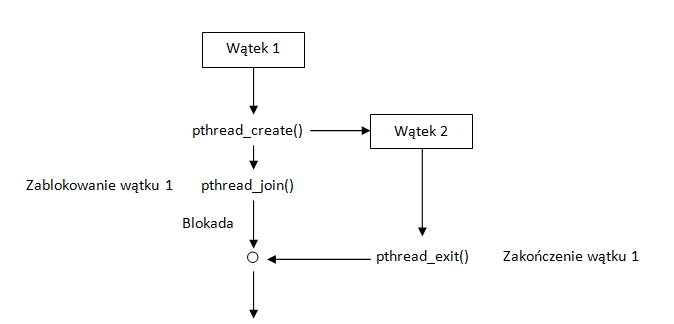
\includegraphics[width=0.85\textwidth]{img/laczenie1}
\caption{Łączenie wątków. Wątek 1 czeka na wątek 2}
\label{fig:laczenie1}
\end{figure}
\begin{figure}[!h]
\centering
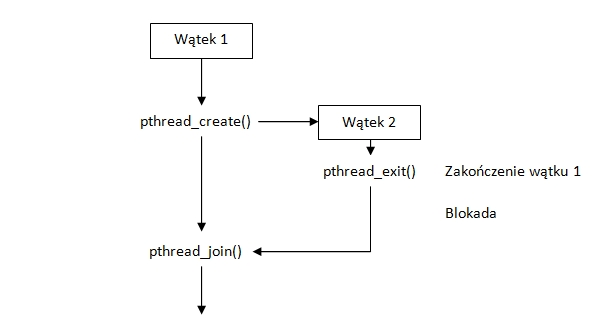
\includegraphics[width=0.85\textwidth]{img/laczenie2}
\caption{Łączenie wątków. Wątek 2 czeka na wątek 1}
\label{fig:laczenie2}
\end{figure}

\begin{example}{[Łączenie wątków]}
Przykład ilustruje omawiane zagadnienia łączenia wątków, wraz z~przekazaniem kodu powrotu z~utworzonych wątków do wątku głównego.

\lstinputlisting[caption=Łączenie wątków,style=MyCStyle,label=src:thirdThread]{src/lab5/thirdThread.c}

\end{example}


\subsubsection{Atrybuty wątków}

Biblioteka \lstinline[style=MyCStyle]{pthread} dostarcza mechanizmu do regulowania własności wątków. Atrybuty wątków są przekazywane jako parametry w~strukturze \lstinline[style=MyCStyle]{pthread_attr_t* attr} funkcji \lstinline[style=MyCStyle]{pthread_create()}, w~chwili tworzenia wątku. W~przypadku, gdy przekazujemy wskaźnik \lstinline[style=MyCStyle]{NULL}, atrybuty są ustawiane domyślnie. Jeśli chcemy utworzyć wątek, z~atrybutami innymi, niż domyślne, jawnie dobranymi przez użytkownika należy:


\begin{myitemize}
\item Utworzyć obiekt \lstinline[style=MyCStyle]{attr} typu \lstinline[style=MyCStyle]{pthread_attr_t}.
\item Zainicjować zmienną \lstinline[style=MyCStyle]{attr} wywołaniem funkcji \lstinline[style=MyCStyle]{pthread_attr_init(&attr)}.
\item Zmodyfikować obiekt z~atrybutami, tak, aby zawierał pożądane wartości.
\item Przekazać wskaźnik do struktury \lstinline[style=MyCStyle]{attr}, w~trakcie tworzenia wątku za pomocą \lstinline[style=MyCStyle]{pthread_create()}.
\item Zwolnić zasoby wykorzystywane przez atrybut, przez wywołanie funkcji \mbox{\lstinline[style=MyCStyle]{pthread_attr_destroy(&attr)}}.
\end{myitemize}

Wybrane atrybuty wątku przedstawiono w tabeli~\ref{tab:atrybuty1}, a~funkcje służące do ich ustawiania w~tabeli~\ref{tab:atrybuty2}.

\begin{table}[h!]
\centering
\caption{Wybrane atrybuty wątku i ich wartości domyślne}
\setlength{\arrayrulewidth}{1pt}
\setlength{\tabcolsep}{6pt}
\renewcommand{\arraystretch}{1.2}
\begin{tabular}{ |p{0.45\textwidth}|p{0.4\textwidth}| }
\hline \rowcolor{gray}
\textbf{Atrybut} & \textbf{Wartość domyślna} \\ \hline
Dołączalność (\mbox{\lstinline[style=MyCStyle]{detachstate}}) & \mbox{\lstinline[style=MyCStyle]{PTHREAD_CREATE_JOINABLE}} \\ \hline
Dziedziczenie atrybutów (\mbox{\lstinline[style=MyCStyle]{inherit-scheduling}}) & \mbox{\lstinline[style=MyCStyle]{PTHREAD_INHERIT_SCHED}} \\ \hline
Strategia szeregowania (\mbox{\lstinline[style=MyCStyle]{schedpolicy}}) & \mbox{\lstinline[style=MyCStyle]{PTHREAD_INHERIT_SCHED}} \\ \hline
Parametry szeregowania (\mbox{\lstinline[style=MyCStyle]{schedparam}}) & Dziedziczone z procesu macierzystego \\ \hline
Rywalizacja wątku o zasoby (\mbox{\lstinline[style=MyCStyle]{contentionscope}}) & \mbox{\lstinline[style=MyCStyle]{PTHREAD_SCOPE_SYSTEM}} \\ \hline
Rozmiar stosu (\mbox{\lstinline[style=MyCStyle]{stacksize}}) & 4kB \\ \hline
Adres stosu (\mbox{\lstinline[style=MyCStyle]{stackaddr}}) & \mbox{\lstinline[style=MyCStyle]{NULL}} \\ \hline
\end{tabular}
\label{tab:atrybuty1}
\end{table}


Objaśnienia:

\begin{myitemize}
\item Dołączalność - informacja, czy wątek ma zwolnić zasoby natychmiast (\lstinline[style=MyCStyle]{PTHREAD_CREATE_DETACHED}), czy po wywołaniu przez proces macierzysty funkcji \lstinline[style=MyCStyle]{pthread_join (PTHREAD_CREATE_JOINABLE)}.
\item Dziedziczenie atrybutów - domyślnie są dziedziczone z~wątku macierzystego.
\item Strategia szeregowania: \lstinline[style=MyCStyle]{SCHED_FIFO}, \lstinline[style=MyCStyle]{SCHED_RR}, \lstinline[style=MyCStyle]{SCHED_SPORADIC}, \lstinline[style=MyCStyle]{SCHED_OTHER} - szczegółowe objaśnienia w~dokumentacji.
\item Parametry szeregowania - informacje, dot. szeregowania wątków. Modyfikowana jest struktura \lstinline[style=MyCStyle]{const struct sched_param * param}.
\item Rywalizacja wątku o~zasoby - wątki mogą rywalizować o~zasoby z~wątkami systemowymi z~innych procesów (ang. system contention scope).  Wątki mogą również rywalizować o~zasoby tylko w~obrębie procesu, który je utworzył (process contention scope). Domyślnie ustawiana jest pierwsza opcja.
\item Rozmiar stosu - informacja o~rozmiarze stosu do przechowywania zmiennych lokalnych.
\item Adres stosu - gdy adres stosu jest ustawiony na \lstinline[style=MyCStyle]{NULL}, to będzie ustalany i~zwalniany automatycznie przez system operacyjny. Pamięć na stos może być też przydzielona przez programistę i~wtedy jest on odpowiedzialny za jej zwolnienie.
\end{myitemize}

Po inicjalizacji struktury z atrybutami, możemy pobierać i ustawiać atrybuty związane z wątkami.

\begin{table}[h!]
\centering
\caption{Funkcje od pobierania i ustawiania atrybutów}
\setlength{\arrayrulewidth}{1pt}
\setlength{\tabcolsep}{6pt}
\renewcommand{\arraystretch}{1.2}
\begin{tabular}{ |p{0.25\textwidth}|p{0.35\textwidth}|p{0.35\textwidth}| }
\hline \rowcolor{gray}
\textbf{Atrybut} & \textbf{Pobierz atrybut} & \textbf{Ustaw atrybut} \\ \hline
Dołączalność & \mbox{\lstinline[style=MyCStyle]{pthread_attr_getdetachstate()}} & \mbox{\lstinline[style=MyCStyle]{pthread_attr_setdetachstate()}} \\ \hline
Dziedziczenie atrybutów & \mbox{\lstinline[style=MyCStyle]{pthread_attr_getinheritsched()}} & \mbox{\lstinline[style=MyCStyle]{pthread_attr_setinheritsched()}} \\ \hline
Strategia szeregowania & \mbox{\lstinline[style=MyCStyle]{pthread_attr_getschedpolicy()}} & \mbox{\lstinline[style=MyCStyle]{pthread_attr_setschedpolicy()}} \\ \hline
Parametry szeregowania & \mbox{\lstinline[style=MyCStyle]{pthread_attr_getschedparam()}} & \mbox{\lstinline[style=MyCStyle]{pthread_attr_setschedparam()}} \\ \hline
Rywalizacja o~zasoby & \mbox{\lstinline[style=MyCStyle]{pthread_attr_getscope()}} & \mbox{\lstinline[style=MyCStyle]{pthread_attr_setscope()}} \\ \hline
Rozmiar stosu & \mbox{\lstinline[style=MyCStyle]{pthread_attr_getstacksize()}} & \mbox{\lstinline[style=MyCStyle]{pthread_attr_setstacksize()}} \\ \hline
Adres stosu & \mbox{\lstinline[style=MyCStyle]{pthread_attr_getstackaddr()}} & \mbox{\lstinline[style=MyCStyle]{pthread_attr_setstackaddr()}} \\ \hline
\end{tabular}
\label{tab:atrybuty2}
\end{table}


\begin{example}{[Atrybuty wątków]}
Przykład ilustruje omawiane zagadnienia łączenia wątków, wraz z~przekazaniem kodu powrotu z~utworzonych wątków do wątku głównego.

\lstinputlisting[caption=Ustawianie atrybutu dołączalności,style=MyCStyle,label=src:attThread]{src/lab5/attThread.c}
\end{example}

\subsubsection{Ustalanie priorytetu, strategii i parametrów szeregowania wątków}


\underline{Dziedziczenie atrybutów}


\noindent\textbf{Ustawianie atrybutów}. Wątki potomne domyślnie dziedziczą priorytet i~własności dotyczące szeregowania z~wątku macierzystego. Funkcja \lstinline[style=MyCStyle]{pthread_attr_setinheritsched} umożliwia zmianę tego stanu:

\begin{lstlisting}[style=MyCStyle]
int pthread_attr_setinheritsched(pthread_attr_t * attr, int inheritsched );
\end{lstlisting}

gdzie \lstinline[style=MyCStyle]{attr} jest wskaźnikiem na strukturę definiującą atrybuty wątku, a~wartość \lstinline[style=MyCStyle]{inheritsched} jest jedną z~dwóch wartości:

\begin{myitemize}
\item \lstinline[style=MyCStyle]{PTHREAD_INHERIT_SCHED} - wątek potomny dziedziczy strategię szeregowania od wątku rodzica - wartość domyślna.
\item \lstinline[style=MyCStyle]{PTHREAD_EXPLICIT_SCHED} - strategia szeregowania jest ustawiona przez strukturę \lstinline[style=MyCStyle]{attr}.
\end{myitemize}

\noindent\textbf{Pobieranie atrybutów}. Funkcją, która umożliwia pobieranie parametrów dot. dziedziczenia własności z~wątku macierzystego ma następującą sygnaturę:

\begin{lstlisting}[style=MyCStyle]
int pthread_attr_getinheritsched(const pthread_attr_t* attr,int* inheritsched );
\end{lstlisting}

gdzie wartość \lstinline[style=MyCStyle]{inheritsched} jest wskaźnikiem do miejsca, gdzie funkcja przechowa atrybut.

\noindent\underline{Strategia szeregowania}

\noindent\textbf{Ustawianie atrybutów}. Ustawianie strategii szeregowania realizujemy funkcją:

\begin{lstlisting}[style=MyCStyle]
int pthread_attr_setschedpolicy(pthread_attr_t* attr, int policy);
\end{lstlisting}

gdzie \lstinline[style=MyCStyle]{attr} jest wskaźnikiem na strukturę definiującą atrybuty wątku, a~wartość \lstinline[style=MyCStyle]{policy} jest jedną z~wartości zdefiniowanych w~tabeli~\ref{tab:sched}.

\begin{table}[h!]
\centering
\caption{Strategie szeregowania w QNX Neutrino}
\setlength{\arrayrulewidth}{1pt}
\setlength{\tabcolsep}{6pt}
\renewcommand{\arraystretch}{1.2}
\begin{tabular}{ |p{0.15\textwidth}|p{0.2\textwidth}|p{0.4\textwidth}| }
\hline \rowcolor{gray}
\textbf{Numer} & \textbf{Symbol} & \textbf{Opis} \\ \hline
\mbox{\lstinline[style=MyCStyle]{0}} & \mbox{\lstinline[style=MyCStyle]{SCHED_NOCHANGE}} & Brak zmiany strategii szeregowania \\ \hline
\mbox{\lstinline[style=MyCStyle]{1}} & \mbox{\lstinline[style=MyCStyle]{SCHED_FIFO}} & Szeregowanie FIFO \\ \hline
\mbox{\lstinline[style=MyCStyle]{2}} & \mbox{\lstinline[style=MyCStyle]{SCHED_RR}} & Szeregowanie karuzelowe \\ \hline
\mbox{\lstinline[style=MyCStyle]{3}} & \mbox{\lstinline[style=MyCStyle]{SCHED_OTHER}} & wskazuje wartość \mbox{\lstinline[style=MyCStyle]{SCHED_RR}} \\ \hline
\mbox{\lstinline[style=MyCStyle]{4}} & \mbox{\lstinline[style=MyCStyle]{SCHED_SPORADIC}} & Szeregowanie sporadyczne \\ \hline
\end{tabular}
\label{tab:sched}
\end{table}

\noindent\textbf{Pobieranie atrybutów}. Pobieranie strategii szeregowania można zrealizować funkcją:

\begin{lstlisting}[style=MyCStyle]
int pthread_attr_getschedpolicy(const pthread_attr_t* attr,int* policy );
\end{lstlisting}

gdzie \lstinline[style=MyCStyle]{policy} jest wskaźnikiem do miejsca przechowywania ustawionej wartości strategii szeregowania.

\noindent\underline{Parametry szeregowania}

\noindent\textbf{Ustawianie atrybutów}. Aby ustawić atrybuty z~tego zbioru należy zastosować funkcję:

\begin{lstlisting}[style=MyCStyle]
int pthread_attr_setschedparam(pthread_attr_t * attr,const struct sched_param * param );
\end{lstlisting}

gdzie \lstinline[style=MyCStyle]{attr} jest wskaźnikiem na strukturę definiującą atrybuty wątku, a~zmienna \lstinline[style=MyCStyle]{param} jest wskaźnikiem na strukturę \lstinline[style=MyCStyle]{sched_param}, która definiuje parametry szeregowania watków.

\noindent\textbf{Pobieranie atrybutów}. Tę funkcję realizujemy następująco:

\begin{lstlisting}[style=MyCStyle]
int pthread_attr_getschedparam(const pthread_attr_t * attr, struct sched_param * param );
\end{lstlisting}

gdzie \lstinline[style=MyCStyle]{param} jest wskaźnikiem na strukturę \lstinline[style=MyCStyle]{sched_param}.

\begin{example}{[Zarządzanie atrybutami szeregowania wątków]}
Przykład pokazuje w~jaki sposób używać atrybutów, w~celu utworzenia wątku ze zdefiniowanymi przez programistę parametrami i~strategią szeregowania.

\lstinputlisting[caption=Pobieranie i ustawianie atrybutów szeregowania wątków,style=MyCStyle,label=src:sched]{src/lab5/sched.c}

Przykładowy wynik działania programu powinien wyglądać następująco:

\begin{lstlisting}[style=MyCStyle]
Priorytet ustawiony przy starcie procesu (watku glownego) 10.
Domyslna strategia ROUND ROBIN, priorytet: 10
Domyslna strategia FIFO, priorytet: 8
Tworze watek z nowymi atrybutami:
	Step = 0
	Step = 1
	Step = 2
	Step = 3
	Step = 4
Watek glowny dolaczyl watek potomny.
Watek glowny zakonczony. Wyjscie.
\end{lstlisting}

\end{example}


\subsection{Ćwiczenia}

\begin{myenumerate}
\item Napisać program, który tworzy $8$ wątków i~przekazuje do niego strukturę następującego typu:

\begin{lstlisting}[style=MyCStyle]
struct thread_data
  {
    int	cnt;          /* numer watku */
    int sum;          /* suma kontrolna */
    const char *msg;  /* wiadomosc */
  }
\end{lstlisting}

gdzie

\begin{myitemize}
  \item \lstinline[style=MyCStyle]{cnt} - numer wątku (nadajemy sami wg kolejności tworzenia: \lstinline[style=MyCStyle]{cnt=0,1,2,...}).
\item \lstinline[style=MyCStyle]{sum} - ,,suma kontrolna'', będąca sumą numerów wątków (np. dla pierwszego wątku \mbox{\lstinline[style=MyCStyle]{sum=0}}, dla drugiego \lstinline[style=MyCStyle]{sum=0+1}, dla trzeciego \lstinline[style=MyCStyle]{sum=0+1+2}, itd.).
\item \lstinline[style=MyCStyle]{msg} - wskaźnik do wiadomości otrzymanej z~programu głównego.
\end{myitemize}

W programie głównym utworzyć tablicę o~następującej zawartości:

\begin{lstlisting}[style=MyCStyle]
messages[0] = "English: Hello World!";
messages[1] = "French: Bonjour, le monde!";
messages[2] = "Spanish: Hola al mundo";
messages[3] = "Polski: Witaj swiecie!";
messages[4] = "German: Guten Tag, Welt!";
messages[5] = "Russian: Zdravstvytye, mir!";
messages[6] = "Japan: Sekai e konnichiwa!";
messages[7] = "Latin: Orbis, te saluto!";
\end{lstlisting}

Odpowiednie pola tablicy będą przekazywane do wątków. Każdy z~wątków powinien wyświetlać otrzymaną strukturę danych. Należy zadbać o~poprawne zakończenie wątków.

\item Zaproponować współbieżną (równoległą - gdy dysponujemy komputerem wieloprocesorowym) wersję programu do obliczania liczby $\pi$ za pomocą wątków. Matematycznie wiadomo, że:

\begin{equation}\nonumber
\displaystyle\int_0^1{\frac{4}{1+x^2}dx}=\pi
\end{equation}

Całkę oznaczoną możemy aproksymować jako sumę:

\begin{equation}\nonumber
\sum_{i=0}^N\frac{4}{1+x_i^2}\Delta x\approx\pi
\end{equation}

Ilustrację graficzną aproksymacji liczby $\pi$ można znaleźć na rysunku~\ref{fig:piApprox}.

\begin{figure}[!h]
\centering
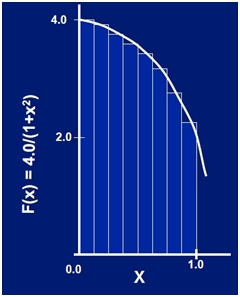
\includegraphics[width=0.4\textwidth]{img/piApprox}
\caption{Idea aproksymacji liczby $\pi$}
\label{fig:piApprox}
\end{figure}

\lstinputlisting[caption=Kod źródłowy sekwencyjnej wersji do obliczania liczby $\pi$,style=MyCStyle,label=src:piApprox]{src/lab5/piApprox.c}

\item Rozszerzyć poprzedni przykład o możliwość zmiany priorytetów i strategii szeregowania wątków.
\end{myenumerate}


\cleardoublepage
